\documentclass{scrreprt}
%\usepackage{float}
\usepackage{fullpage}
\usepackage{caption}
\usepackage{subcaption}
\usepackage{listings}
\usepackage{underscore}
\usepackage{tabularx}
\usepackage{longtable}
\usepackage{graphicx}
\usepackage[bookmarks=true]{hyperref}
\usepackage{pdfpages}
\usepackage{cite}

\hypersetup{
%    bookmarks=false,    % show bookmarks bar?
    pdftitle={Software Requirement Specification},    % title
    pdfauthor={Homer J. Simpson},                     % author
    pdfsubject={TeX and LaTeX},                        % subject of the document
    pdfkeywords={TeX, LaTeX, graphics, images}, % list of keywords
    colorlinks=true,       % false: boxed links; true: colored links
    linkcolor=blue,       % color of internal links
    citecolor=black,       % color of links to bibliography
    filecolor=black,        % color of file links
    urlcolor=purple,        % color of external links
    linktoc=page            % only page is linked
}

\def\myversion{1.0 }

\newcounter{myCounter}[subsection] 
\newcounter{mySubCounter}[myCounter] 

\makeatletter
\newcommand{\reqLabel}[1]{%
\myLabel{#1}{Req}}
\makeatother

\makeatletter
\newcommand{\reqLabelB}[1]{%
\myLabelB{#1}{Req}}
\makeatother

\makeatletter
\newcommand{\specLabel}[1]{%
\myLabel{#1}{Spec}}
\makeatother

\makeatletter
\newcommand{\specLabelB}[1]{%
\myLabelB{#1}{Spec}}
\makeatother

\makeatletter
\newcommand{\defLabel}[1]{%
\myLabel{#1}{Def}}
\makeatother

\makeatletter
\newcommand{\nfLabel}[1]{%
\myLabel{#1}{NF}}
\makeatother

%%%%%%%%%%%%%%%%%%%%%%%%%%%%%%%%%% Variante 1 %%%%%%%%%%%%%%%%%%%%%%%%%%%%%%%%%%%%%%%
\newcommand{\layerOne}[1]{\chapter{#1}}
\newcommand{\layerOneStar}[1]{\chapter*{#1}}
\newcommand{\layerTwo}[1]{\section{#1}}
\newcommand{\layerThree}[1]{\subsection{#1}}
\newcommand{\layerFour}[1]{\subsubsection{#1}}

\makeatletter
	\newcommand{\myLabel}[2]{%
		\refstepcounter{myCounter}
		\def\@currentlabel{#2-\thesubsection.\arabic{myCounter}}% Update label
		\raisebox{\f@size pt}\phantomsection
		\label{req:#1}
		#2-\thesubsection.\arabic{myCounter}}
\makeatother

%\makeatletter
%	\newcommand{\myLabelFour}[2]{%
%		\refstepcounter{myCounter}
%		\def\@currentlabel{#2-\thesubsection.\arabic{myCounter}}% Update label
%		\raisebox{\f@size pt}\phantomsection
%		\label{req:#1}
%		#2-\thesubsection.\arabic{myCounter}}
%\makeatother

\newcommand{\kmh}{$kmh^{-1}$}

\makeatletter
	\newcommand{\myLabelB}[2]{%
		\refstepcounter{mySubCounter}
		\def\@currentlabel{#2-\thesubsection.\arabic{myCounter}\alph{mySubCounter}}% Update label
		\raisebox{\f@size pt}\phantomsection
		\label{req:#1}
		#2-\thesubsection.\arabic{myCounter}\alph{mySubCounter}}
\makeatother

%%%%%%%%%%%%%%%%%%%%%%%%%%%%%%%%%% Variante 2 %%%%%%%%%%%%%%%%%%%%%%%%%%%%%%%%%%%%%%%
%
%\newcommand{\layerOne}[1]{\part{#1}}
%\newcommand{\layerOneStar}[1]{\part*{#1}}
%\newcommand{\layerTwo}[1]{\chapter{#1}}
%\newcommand{\layerThree}[1]{\section{#1}}
%
%\makeatletter
%	\newcommand{\myLabel}[2]{%
%		\refstepcounter{myCounter}
%		\def\@currentlabel{#2-\thesubsection.\arabic{myCounter}}% Update label
%		\raisebox{\f@size pt}\phantomsection
%		\label{req:#1}
%		#2-\thesubsection.\arabic{myCounter}}
%\makeatother
%
%\makeatletter
%	\newcommand{\myLabelB}[2]{%
%		\refstepcounter{mySubCounter}
%		\def\@currentlabel{#2-\thesubsection.\arabic{myCounter}\alph{mySubCounter}}% Update label
%		\raisebox{\f@size pt}\phantomsection
%		\label{req:#1}
%		#2-\thesubsection.\arabic{myCounter}\alph{mySubCounter}}
%\makeatother
%
%%%%%%%%%%%%%%%%%%%%%%%%%%%%%%%%%% Variante Ende %%%%%%%%%%%%%%%%%%%%%%%%%%%%%%%%%%%%%%%

\makeatletter
  \newcommand{\myRef}[1]{
  \ref{req:#1}}
\makeatother

\makeatletter
  \newcommand{\comment}{
  \hspace{1em} \textit{Comment}}
\makeatother


\title{
\flushright
\rule{16cm}{5pt}\vskip1cm
\Huge{SOFTWARE REQUIREMENTS\\ SPECIFICATION}\\
\vspace{2cm}
for a\\
\vspace{2cm}
Train Control System\\
\vspace{2cm}
\LARGE{Release 1.0\\}
\vspace{2cm}
\LARGE{Version \myversion approved\\}
\vfill
\rule{16cm}{5pt}
}
\date{}
\usepackage{hyperref}
\begin{document}
\maketitle
%\includepdf[pages=1]{img/title.pdf}
\newpage
\phantomsection
\addcontentsline{toc}{chapter}{Contents}

\tableofcontents

\clearpage
\phantomsection
\addcontentsline{toc}{chapter}{Revision History}
\layerOneStar{Revision History}

\layerOne{Requirements} 

\begin{tabularx}{\textwidth}[t]{|l|X|} \hline
\reqLabel{general:r1} & Some requirements may be optional. \myRef{general:s1}\\ \hline
\end{tabularx}

\layerTwo{XMF-Language}
\layerTwo{Kernel}
\layerTwo{X-Modeler}

\layerThree{Diagrams}

\layerFour{Multi-Level Diagram}

\layerOne{Specifications} 

\setcounter{myCounter}{0}
\begin{tabularx}{\textwidth}[t]{|l|X|} \hline
\reqLabel{general:s1} & Some specifications may be optional. \myRef{general:r1}\\ \hline
\end{tabularx}

\layerTwo{XMF-Language}
\layerTwo{Kernel}
\layerTwo{X-Modeler}

\layerThree{Diagrams}

\layerFour{Multi-Level Diagram}

\layerThree{Signals}

\begin{tabularx}{\textwidth}[t]{|l|X|}
	  \hline
    \specLabel{signal:hp0} & Hp0: Stop aspect. One or two red lights. See Fig.~\ref{fig:hp012}, \myRef{signal:1}, \myRef{signal:1a} \\	\hline
		\specLabel{signal:hp1} & Hp1: Proceed aspect. One green light. See Fig.~\ref{fig:hp012}, \myRef{signal:1}\\ \hline
		\specLabel{signal:hp2} & Hp2: Slow aspect. One green over one yellow light. Shown for speeds up to $60kmh^{-1}$. If no speed is specified by Zs3 the limit is $40kmh^{-1}$. 
		This default speed limit may be changed to $50kmh^{-1}$ or $60kmh^{-1}$. 
		See Fig.~\ref{fig:hp012}, \myRef{signal:1}, \myRef{signal:zs3}, \myRef{editor:signal:s3:L5Ma}, \myRef{editor:signal:s3:L5Mb},
		\myRef{editor:signal:s3:L5Mc}, \myRef{editor:signal:s3:L5Md}, \myRef{editor:signal:s3:L6Ma}  \\ \hline
\end{tabularx}

\vspace{.5cm}
\begin{figure}[ht!]
	\centering
	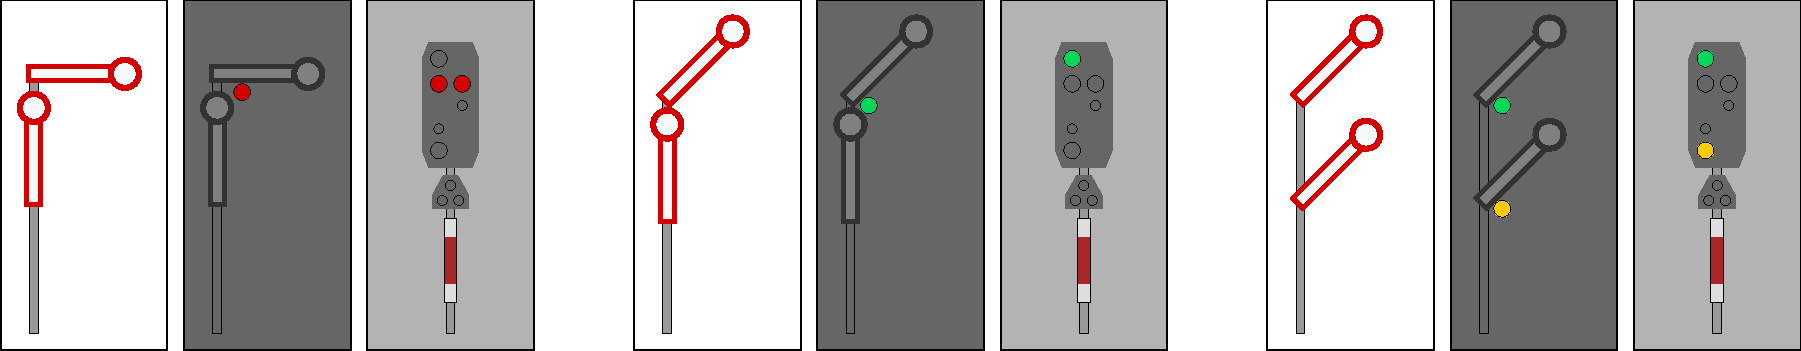
\includegraphics[width=420pt]{img/hp012.pdf}
	\caption{from left to right: Hp0, Hp1, Hp2}
	\label{fig:hp012}
\end{figure}

%\noindent

\nocite{*}

\clearpage
\phantomsection
\addcontentsline{toc}{chapter}{Bibliography}
\bibliography{literatur}
\bibliographystyle{literaturStyle}
\end{document}
